\documentclass[11pt]{beamer}
\usetheme{default}

\usepackage[utf8]{inputenc}
\usepackage[english]{babel}
\usepackage{amsmath}
\usepackage{amsfonts}
\usepackage{amssymb}
\usepackage{graphicx}
\usetheme{Luebeck}

\author{hk}
\title{testpres}

%subtitle{}
%
%logo{}
%
%institute{}
%
%date{}
%
%subject{}
%
%setbeamercovered{transparent}
%
%setbeamertemplate{navigation symbols}{}

\begin{document}
	
	\begin{frame}
		\frametitle{}
	\end{frame}
	
	\begin{frame}{Introduction}
		First Slide
	\end{frame}
	
	\begin{frame}{A Picture}
		\begin{figure}
			\centering
			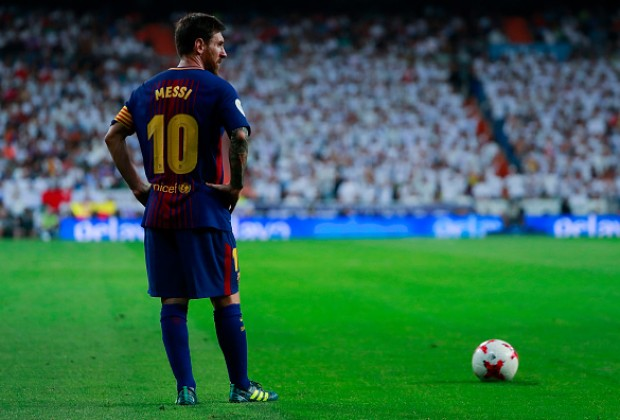
\includegraphics[width=0.9\linewidth]{messi.jpg}
		\end{figure}
	\end{frame}
	
	\begin{frame}{Lists}
		\begin{enumerate}
			\item apple
			\item orange
			\item banana
		\end{enumerate}
	\end{frame}	
	\begin{frame}{One simple equation}
		$$ y^2 = x^{n+1} + \frac{13}{17}$$
	\end{frame}	
	
	\begin{frame}{One table about grades}
		\begin{center}
		    \begin{tabular}{|c|c|c|}
		    	\hline
		        a & b & c \\
		        \hline
		    \end{tabular}
		\end{center}
	\end{frame}		
\end{document}